%%% Fiktivní kapitola s ukázkami sazby

\chapter{Problémová oblast}{\tiny }

% https://www.euppublishing.com/doi/10.3366/anh.2018.0487
% https://web.archive.org/web/20110724161954/http://ardeajournal.natuurinfo.nl/ardeapdf/a89-001-006.pdf
% http://krouzkovaniptaku.cz/historie/

Sledování ptačích migrací je poměrně starou vědeckou disciplínou s kořeny v roce 1805. Americký ornitolog John James Audubon se snažil prokázat, že se každým rokem na jeho farmu vrací stejný jedinec druhu \emph{Sayornis phoebe} přivázáním stříbrného lanka na nohu. Tímto nepřímo položil základy pro tzv. kroužkování, pasivní označení jedinců kovovým kroužkem s vyraženým sériovým identifikátorem kroužku. Systém kroužkování zavedl dánský ornitolog a učitel Hans Christian Cornelius Mortensen v roku 1899. Na území České republiky se kroužkování ujalo roku 1910, přibližně rok po rozšíření systému v Anglii a Německu. Mezinárodní kolaborací ornitologů se tzv. odečítáním kroužků podařilo zmapovat migrační trasy mnoha ptačích druhů. 

% https://www.fs.fed.us/t-d/programs/im/satellite_gps_telemetry/wildlifetrackingtelementry.htm

Miniaturizací elektronických součástek, především akumulátorů, se v 60. letech 20. století začínají rozšiřovat aktivní telemetrická zařízení. Jednoduché radiolokátory umožnily v terénu přesně určit pozici zvířete sledováním intenzity signálu. Radiolokátory mohou pomocí elektromagnetických pulsů přenášet určitá data (např. identifikátor radiolokátoru -- zvířete) za použití určité modulace signálu. Tímto se zjednodušilo např. hledání hnízd, čímž se taktéž usnadnilo hledání a označení mladých jedinců, kteří ještě nebyli vyvedeni z hnízda.

% https://en.wikipedia.org/wiki/GPS_wildlife_tracking

Ornitologie těžila i z rozvoje kosmických programů. Signály z dostatečně výkonných radiolokátorů mohou být přijaty speciálními družicemi v kosmu a za pomocí Dopplerova jevu lze spočítat přibližnou polohu daného jedince. Tato řešení nebyla zpočátku pro ornitologii příliš vhodná z hlediska hmotnosti radiolokátorů. Příchodem GSM sítí v 90. letech a uvolňování restrikcí na použití GPS se situace pro ornitology zásadně změnila. Na trhu se objevily výrazně lehčí (desítky až jednotky gramů) GPS-GSM trackery vhodné i pro malé druhy ptáků. Data z těchto trackerů se průběžně sbírají a odesílají do systémů výrobců zařízení, případně přímo majiteli zařízení.

Rapidní nástup webových technologií po roce 2000 umožňil výrobcům zařízení jednoduše uživatelům poskytovat navazující služby ke svým zařízením, jmenovitě jednoduchou konfiguraci zařízení, základní visualizaci dat, exporty dat, vedení metainformací k zařízení (např. na jakém zvířeti zařízení je) a další. Většina systémů se omezuje pouze na trackery od jednoho výrobce a funkce mimo množinu konfigurace zařízení jsou primitivní, až nedostatečné. V roce 20?? vznikla česká ornitologická platforma Anitra, která poskytuje komplexní nástroje pro správu zařízení a visualizaci dat od širokého spektra výrobců trackerů. Platforma Anitra taktéž poskytuje správu metainformací o zvířetech, správu zájmových bodů, nahrávání příloh a komplexní metody sdílení dat. Pro tuto práci byla platforma Anitra vybraná z důvodu autorovy možnosti vytvářet API na míru mobilní aplikaci a již existující uživatelské základny.

Pro základní představu celého systému je níže uvedeno schématické znázornění vztahů mezi jeho prvky.

\begin{figure}
	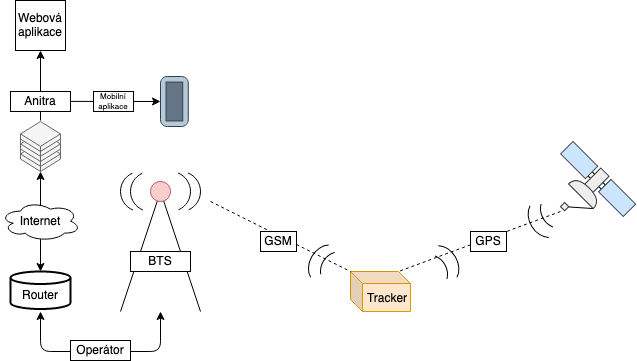
\includegraphics[width=\linewidth]{img/diagram_system.png}
	\caption{Schéma systému GPS-GSM trackerů}
	\label{fig:boat1}
\end{figure}